\documentclass[a4paper,10pt]{article}
\usepackage[utf8]{inputenc}
\usepackage[pdftex]{graphicx}
\usepackage{listings}

%opening
\title{Monitor documentation}
\author{\small {Vennier Manuel}}

\begin{document}
\lstset{language=C++}
\maketitle

\section{Possibilities}

With a monitor, you can see the positions, velocities, forces of chosen particles directly in the GUI or save it into files (readable with Gnuplot)\\
(See \textbf{Figure \ref{figure1} } to look at a monitor in action)

\section{How to add a monitor to your scene}

\begin{enumerate}
	\item In a XML file :\\
	Simply write ``Monitor'' for the \textit{type} field; type ``ExportPositions'', ``ExportVelocities'' or ``ExportForces''
	to true if you want to export positions, velocities or forces in files (Can also be done after in the GUI).
	Finally, to tell which particle(s) you want to monitor, type ``MonitoredParticles'' followed by :\\

	P\textit{``number of positions to monitor, 0 if none''} [\textit{``indices of the particles''}] \\
	V\textit{``number of velocities to monitor, 0 if none''} [\textit{``indices of the particles''}] \\
	F\textit{``number of forces to monitor, 0 if none''} [\textit{``indices of the particles''}] \\

	For example :
	P3 [12 4 0] V0 [] F5 [1 2 3 4 5]

	You can also see the ``monitoredBeamSpring.scn'' file for an example (located in the \textit{examples/Components/monitor} directory)

	\item In a c++ file :\\
	Include first the Monitor header located in \textit{sofa/component/misc/}.
	You must then define three vectors which will contain the indices :

\begin{lstlisting}
sofa::helper::vector <int> posIndices;
sofa::helper::vector <int> velsIndices;
sofa::helper::vector <int> forcesIndices;
\end{lstlisting}

	then add to the vectors the indices of particles you want to monitor (with the $push\_back$ function)

	Finally, give those vectors to the monitor with the following member functions :

\begin{lstlisting}
void setIndPos (sofa::helper::vector <int>);
void setIndVels (sofa::helper::vector <int>);
void setIndForces (sofa::helper::vector <int>);
\end{lstlisting}

\section{Interact with the monitor}

Once the scene launched, if you click on the monitor node in the graph, you should have something like :


	\begin{figure} [h]
	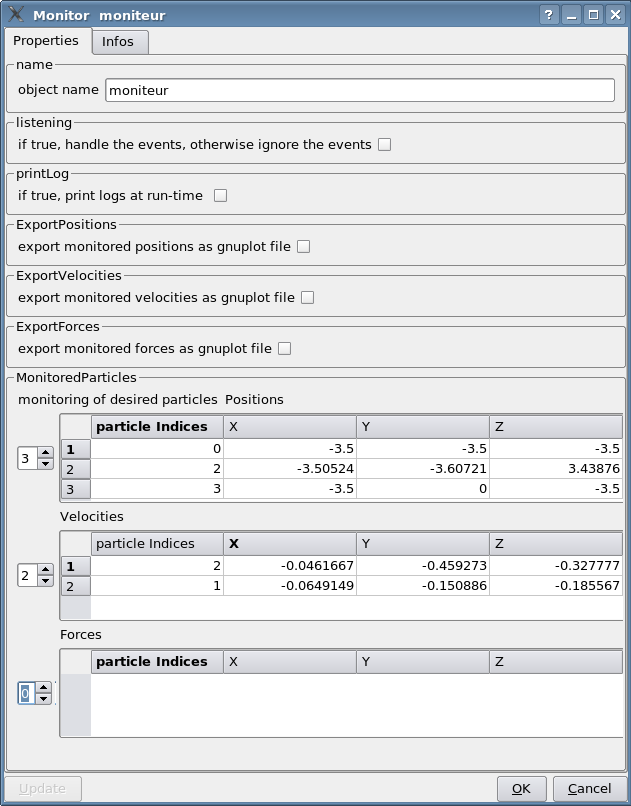
\includegraphics[scale=0.5] {QTableMonitor.png}
	\caption{Example of monitoring tab}
	\label{figure1}
	\end{figure}


By clicking on one of the \textit{particle Indices} boxes, you can change the number of the particle monitored.
With the \textit{spinBox} on the left, you can add or remove particles to monitor.





\end{enumerate}


\end{document}
